\documentclass{beamer}
\usetheme{Warsaw}

\title{Rule Based Grammar Checker For Pashto Language} \vspace{1em}
\author[1]{\textbf {Mustafa Toufiq} \\ P157001@nu.edu.pk \\ \vspace{1.5em} MS(Computer Science)\\ \vspace{1.5em} \textbf{Supervisor: Associate Professor Dr.Omar Usman Khan}\\ omar.khan@nu.edu.pk}
\institute{\textbf{National University of Computer and Emerging Sciences}}
\usepackage{graphicx}
\graphicspath{ {C:/Users/Mustafa/Desktop/Thesis/} }

%\setbeamertemplate{footline}[frame number]
\newcommand*\oldmacro{}%
\let\oldmacro\insertshorttitle%
\renewcommand*\insertshorttitle{%
	\oldmacro\hfill%
	\insertframenumber\,/\,\inserttotalframenumber}
\begin{document}
\thispagestyle{empty}
\setcounter{page}{1}
\newpage


\newcounter{saveenumi}
\newcommand{\seti}{\setcounter{saveenumi}{\value{enumi}}}
\newcommand{\conti}{\setcounter{enumi}{\value{saveenumi}}}


	
\begin{frame}
\titlepage
\end{frame}


\begin{frame}{Contents}
\begin{itemize}
\item Introduction
\vspace{0.3em}
\item Literature Review
\vspace{0.3em}
\item Rule Based Method
\vspace{0.3em}
\item Problem Statement
\vspace{0.3em}
\item Methodology
\vspace{0.3em}
\item Progress
\vspace{0.3em}
\item Future Work
\vspace{0.3em}
\item References
\end{itemize}
\end{frame}


\begin{frame}{Introduction}
\textbf{Area of Research:} Natural Language Processing (NLP) \\
\vspace{1em}
\textbf{Topic of Research:} Rule Based Grammar Checker For Pashto \\ \vspace{0.2em} \hspace{3.3cm} Language.
\end{frame}


\begin{frame}{Background}
\begin{block}{Grammar Checker}
\vspace{0.5em}
A \textbf {Grammar Checker} program allows us to correct a mistake while the
word or phrase is still fresh in our mind.
\vspace{0.5em}	
\end{block}
\end{frame}


\begin{frame}{Literature Review}
\begin{itemize}
	\item \textbf{Statistical Based Approach} \\
	\vspace{1em}
	\begin{itemize}
		\item A POS-annotated corpus is used to build a list of POS tag sequences.\\
		\vspace{0.8em}
		\item Some sequences will be very common, others will probably not occur at all. \\
		\vspace{0.8em}
		\item Sequences which occur	often in the corpus can be considered correct while uncommon sequences could be errors. 
	\end{itemize}
\end{itemize}
	\vspace{4em}
	\footnotesize \color{blue}Asanilta Fahda Ayu Purwarianti 
	\color{black} {"A Statistical and Rule-Based Spelling and Grammar Checker for Indonesian Text"}\\
	\color{blue} International Conference on data and software engineering Indonesia(2017)
\end{frame}


\begin{frame}{Literature Review}
	\begin{itemize}
		\item \textbf{Example}
\begin{center}
	\includegraphics[scale=0.8]{Screenshot_2.png}	
\end{center}
\vspace{3em}
\end{itemize}
\end{frame}



\begin{frame}{Literature Review}
\begin{itemize}
\item \textbf{Statistical Based Approach} \\
\vspace{0.5em}
\begin{itemize}
	\item \textbf{Difficult to interpret:} 
	\vspace{1em}
	\begin{itemize}
		\item If the system raises false errors, users will wonder why their input is considered incorrect when no specific error message is given be errors. 
	\end{itemize}
	\vspace{5em}
\footnotesize \color{blue}Khaled F. Shaalan
\color{black} {"Arabic GramCheck:	A grammar checker for Arabic"} \\
\color{blue} Wiley InterScience(2005)	
\end{itemize}
\end{itemize}
\end{frame}


\begin{frame}{Literature Review}
\begin{itemize}
	\vspace{2em}
	\item \textbf{Statistical and Rule-Based Approach} \\
	\vspace{1em}
	\begin{enumerate}
		\item Statistics-based approach is used for sentence structure which are usually more complex. \\
		\vspace{1em}
		\item Rule-based approach is used for handling most common errors.   \\ 
		%\vspace{0.5em}
		\begin{itemize}
			\item Errors like mechanic editing or ognitive errors.\\	
		\end{itemize}
		\vspace{4em}
	\end{enumerate}
	\footnotesize \color{blue}Asanilta Fahda Ayu Purwarianti 
	\color{black} {"A Statistical and Rule-Based Spelling and Grammar Checker for Indonesian Text"}\\
	\color{blue} International Conference on data and software engineering Indonesia(2017)
\end{itemize}
\end{frame}



\begin{frame}{Literature Review}
\begin{itemize}
	\vspace{0.5em}
	\item \textbf{Two Pass Parsing Implementation for an Urdu Grammar Checker} \\
	\vspace{1em}
	\begin{itemize}
		\item A sentence is first parsed on basic PSG (Phrase Structure Grammar) rules.  \\
		\vspace{0.5em}
		\item Upon failure, Movement Rules are applied to convert it to a desired correct form. \\ 
		\begin{itemize}
			\item It helps in reducing the number of PSR needed to represent the sentence.
		\end{itemize}
		\vspace{0.5em}
		\item After that the sentence is reparsed to check for errors.\\
		\vspace{2em}	
	\end{itemize}
	\footnotesize \color{blue}Hammad Kabir, Shanza Nayyer, Jahangir Zaman, and Dr. Sarmad Hussain
	\color{black} {"Two Pass Parsing Implementation for an Urdu Grammar Checker"} 
	\color{blue} Inmic(2002), Karachi
\end{itemize}
\end{frame}


%\begin{frame}{Literature Review}
%\begin{center}
%	\begin{itemize}
%		\item \textbf{PSG Example} \\
%	\end{itemize}
%\end{center}
%\hspace{1em}
%\includegraphics[scale=0.55]{Screenshot_3.png}	
%\hspace{4em}
%\includegraphics[scale=0.6]{Screenshot_9.jpg}
%\end{frame}



\begin{frame}{Flow Chart of Urdu Grammar Checker}
\begin{center}
	\includegraphics[scale=0.6]{Screenshot_6.jpg}	
\end{center}
\end{frame}


\begin{frame}{Rule Based Grammar Checker}
	\begin{itemize}
	\item  A POS-annotated corpus is used to build a list of POS tag sequences. \\
	\vspace{1em}
	\item  Input text is tokenized and every word is assigned with its POS tag. \\
	\vspace{1em}
	\item  Some base rules are made to generate different trees as a result a tree-bank is created.  \\
	\vspace{1em} 
	\item  The input sentence is then checked with the tree bank. \\
	\vspace{1em}
	\item  If parsing is successful, the sentence will be marked as correct. \\
	\vspace{1em}
	\item  Else it will go to the next module which is error detection and suggestion.
	\end{itemize}
\end{frame}


\begin{frame}{Rule Based Grammar Checker}
\begin{center}
	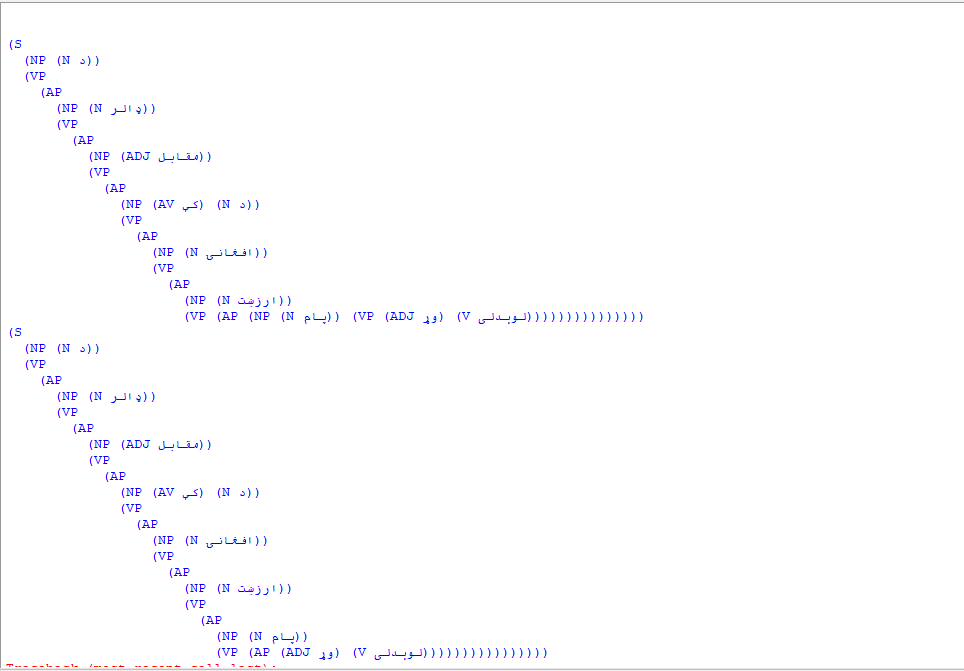
\includegraphics[scale=0.22]{2.png}	
\end{center}
\end{frame}




\begin{frame}{Probabilistic Production Rules}
	\begin{itemize}
	\item  All of the production rules are made from different Pashto sentences. \\
	\vspace{1em}
	\item  Total 40 production rules are used in order to train our system. \\
	\vspace{1em}
	\item  All of the production rules consist of some probability (between 0 to 1).  \\
	\vspace{1em} 
	\item  After training different parse trees can be generated for different sentences. \\
	\vspace{1em}
	\item  Tree Generated = Sentence grammatically correct.\\
		Else = Sentence grammatically incorrect. \\
	\vspace{1em}
	\end{itemize}
\end{frame}



\begin{frame}{Probabilistic Production Rule}
\begin{center}
	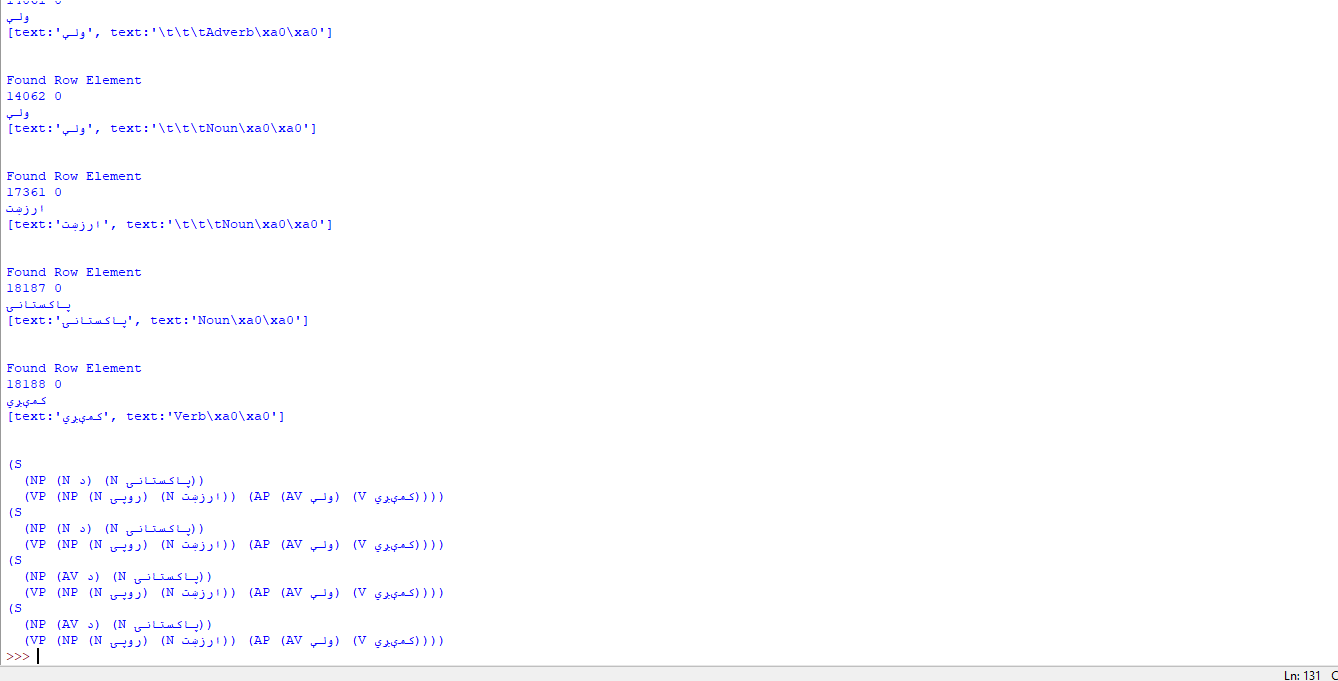
\includegraphics[scale=0.9]{1.png}	
\end{center}
\end{frame}




\begin{frame}{DataSet (Corpus)}
\begin{itemize}
	\item Two types of datasets are used. \\
	\vspace{0.5em}
	\begin{enumerate}
	\item For Testing.
	\item For Training.
	\end{enumerate}
	\vspace{1em}
	\item Training Dataset = 25 sentences (for creation of production rules).
	\item Testing Dataset = 50 sentences (for testing)
	\vspace{1em} 
\end{itemize}
\end{frame}



\begin{frame}{Statistics}
\begin{center}
	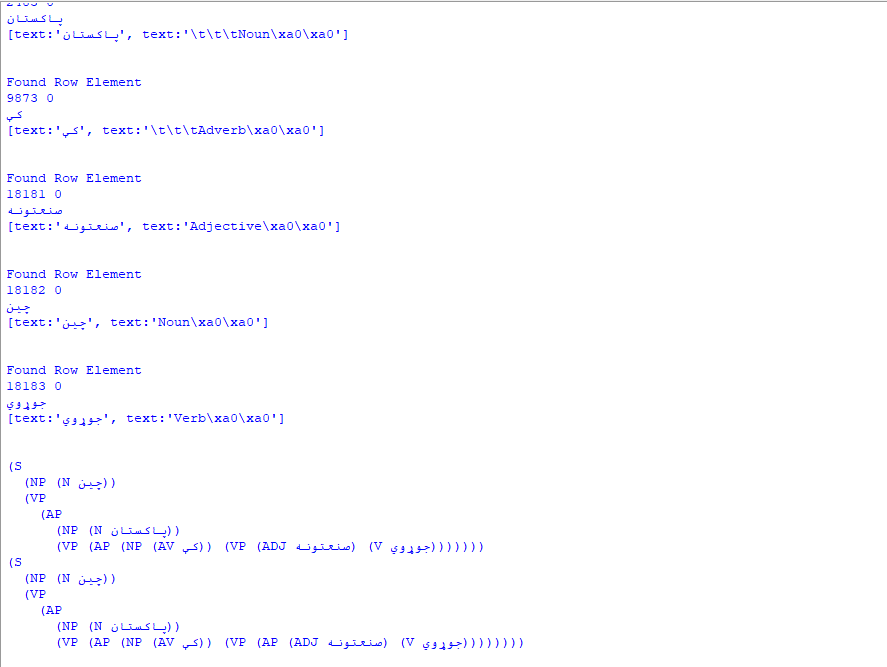
\includegraphics[scale=0.6]{22.png}	
\end{center}
\end{frame}




\begin{frame}{Parsers}
\begin{itemize}
	\item Initially we applied two parsers. \\
	\vspace{0.5em}
	\begin{enumerate}
	\item Shift Reduce Parser.
	\item Recursive Decent Parser.
	\end{enumerate}
	\vspace{1em}
	\item  \textbf{Problems with these parsers}. \\
	\vspace{0.5em}
	\begin{itemize}
	\item Infinite loop.
	\item Exponential time.
	\end{itemize}
	\vspace{1em}
	\item \textbf{Solution}
	\vspace{0.5em}
	\begin{itemize}
	\item Chat Parser.
	\end{itemize}	
	\vspace{1em} 
\end{itemize}
\end{frame}





\begin{frame}{Chart Parser}
\begin{itemize}
	\item Chart or matrix size N + 1, (N = number of words in the input). \\
	\vspace{0.5em}
	\item left-to-right Parser.
	\vspace{0.5em}
	\item Generates partial parse trees.
	\vspace{0.5em}
	\item \textbf{3 States:}
	\begin{enumerate}
	\item Completed constituents; VP -> V NP •
	\item In-progress constituents; NP -> Det • Nom
	\item Predicted constituents; S -> • VP
	\end{enumerate}
	\vspace{1em}
	\item We add a pair of \textbf{coordinates [x, y]} to the state: \\
	\vspace{0.5em}
	\item A -> infinity [x, y]  (x= position in input where the state begins \\
				\hspace{0.5em}	y= position of dot)
	                             
\end{itemize}
\end{frame}



\begin{frame}{Example}
\begin{center}
	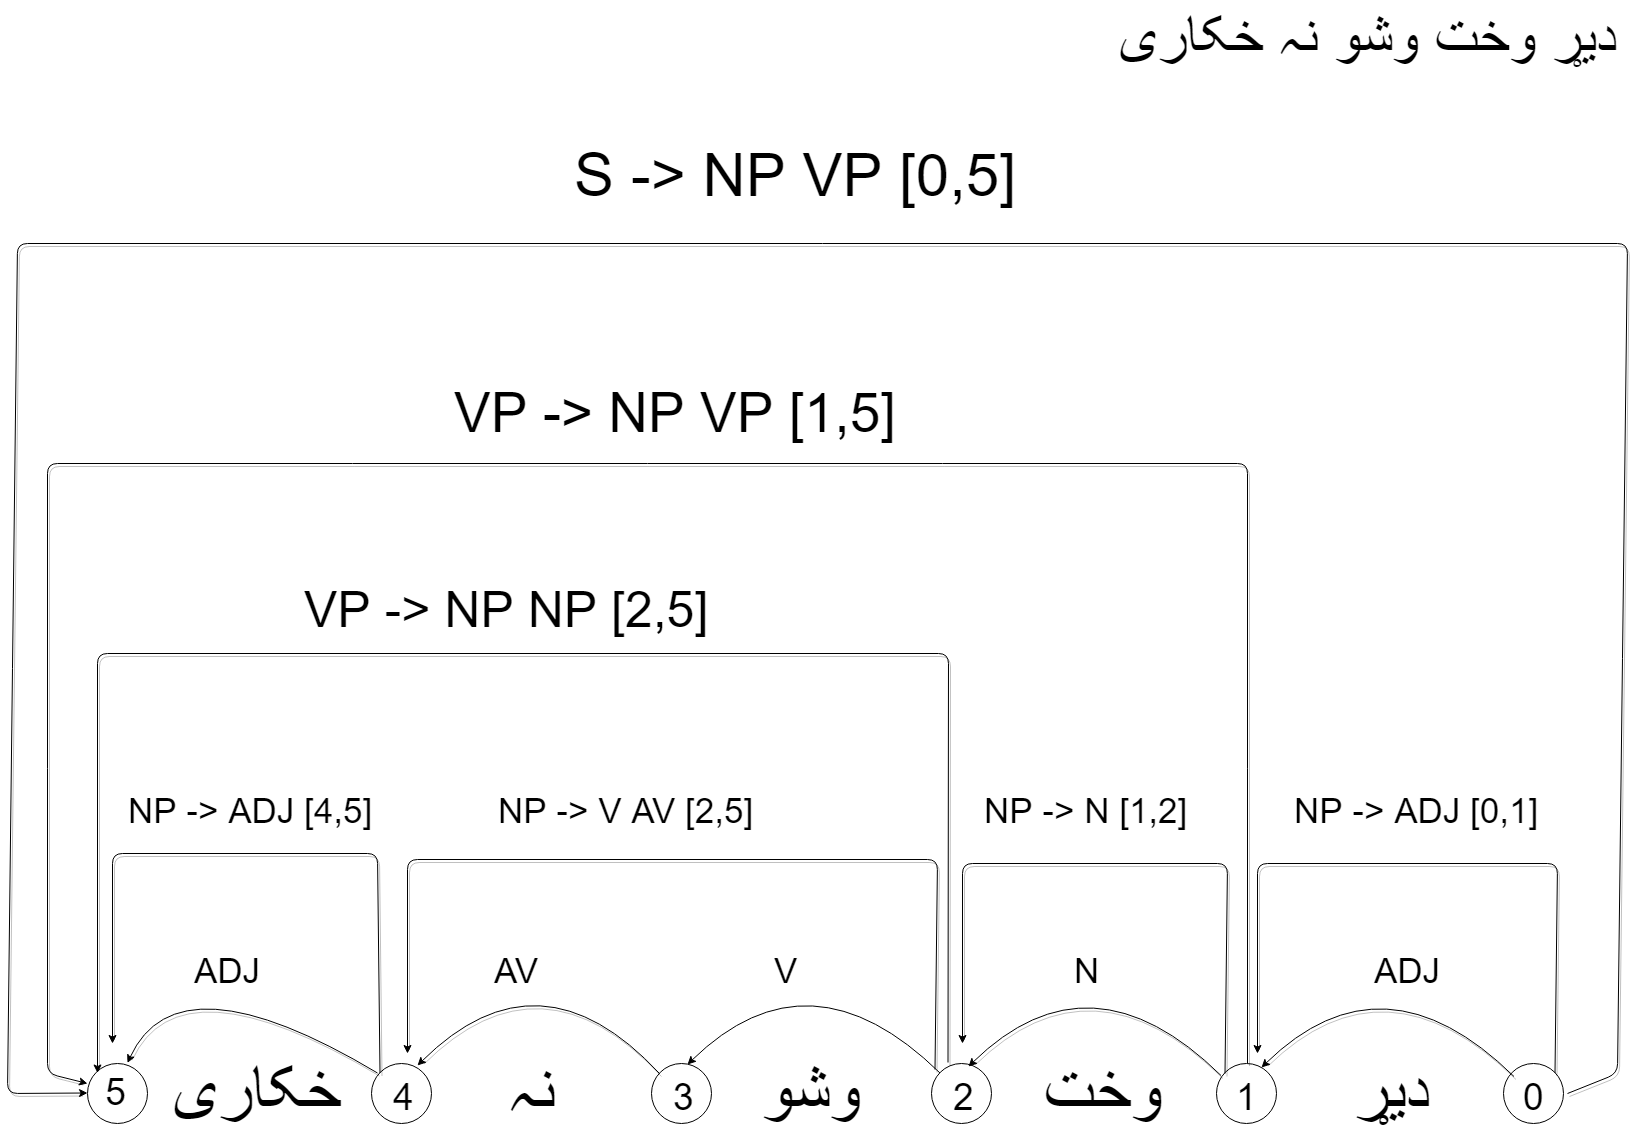
\includegraphics[scale=0.18]{45.png}	
\end{center}
\end{frame}




\begin{frame}{Assigning Probabilities}
\begin{itemize}
	\item All the production rules consits of some probabilities. \\
	\vspace{0.5em}
	\item In order to assign probability to a rule we first check the transition frequency.
	\vspace{0.5em}
	\item Transition frequencies are generated from the training dataset.
	\vspace{0.5em}	                             
\end{itemize}
\end{frame}


\begin{frame}{State Transition Diagram}
\begin{center}
	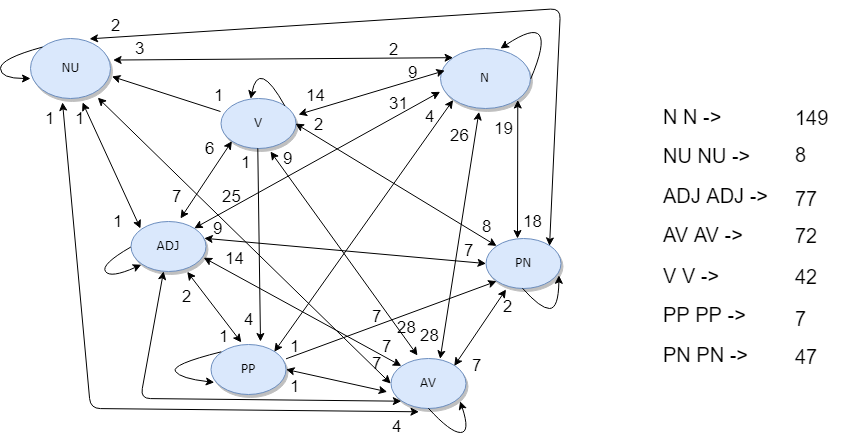
\includegraphics[scale=0.4]{44.png}	
\end{center}
\end{frame}



\begin{frame}{Future Work}
\begin{enumerate}	
	\item Creation of a Tree Bank.  
	\vspace{1em}
	\item After we obtain all the trees we will create a tree bank
	\vspace{1em}
	\item Tree bank will only contain the trees having maximum probability.
\end{enumerate}
\end{frame}




%\begin{frame}{Recursive Decent Parser}
%\begin{itemize}
%	\item It interprets a grammar as how to break complete sentence into several different words. \\
%	\vspace{1em}
%	\item  First it will break a sentence S into two parts  S -> NP VP. \\
%	\vspace{1em}
%	\item  Production permits the parser to replace S with two subgoals: find an NP, then find a VP in production rules.  \\
%	\vspace{1em} 
%	\item  Eventually, this expansion process leads to finding a specific terminal e.g the word "telescope". \\
%	\vspace{1em}
%	\item   This way the production rules can be directly compared against the input sequence. \\
%\end{itemize}
%\end{frame}


%\begin{frame}{Shift Reduce Parser}
%\begin{itemize}
%	\item \textbf{Basic Operations}
%	\vspace{1em}
%	\begin{itemize}
%		\item \textbf{Shift:} Moves symbols from input buffer onto the stack. \\
%		\vspace{1em}
%		\item \textbf{Reduce:} If the top n items on the stack match the n items on the RHS of some production, they are all popped off the stack and the item on the LHS is pushed on the stack. \\ % This replacement of the top n items with a single item is the reduce operation. \\
%		\vspace{1em}
%		\item \textbf{Accept:} If only start symbol is present in the stack and the input buffer is empty, the parsing is called accept. When accept action is obtained, parsing is done successfully\\
%		\vspace{1em} 
%		\item \textbf{Error:} When parser can neither perform shift nor reduce and not even accept action. \\
%		\vspace{1em}
%			\end{itemize}
%	\end{itemize}
%	\footnotesize \color{blue}	Stuart M. Shieber
%\color{black} {"Sentence disambiguation by a shift-reduce parsing technique"} 
%\color{blue} ACL(1983), Cambridge, Massachusetts
%\end{frame}





\begin{frame}{Problem Statement}
\begin{itemize}
\item  No \textbf{Rule Based} Grammar Checker is available for \textbf{Pashto Language} which can identify grammatical mistakes.
\end{itemize}
\end{frame}


\begin{frame}{Methodology}
\begin{itemize}
	\item Creating a POS tagger and developing a tree-bank with the help of which we can identify grammatical errors in a sentence and give suggestions,
\end{itemize}
\end{frame}


\begin{frame}{References}
\begin{enumerate}
\item \color{blue}Khaled F. Shaalan
	\color{black} {"Arabic GramCheck:	A grammar checker for Arabic"} \\
	\color{blue} Wiley InterScience(2005)
	\vspace{2em}
	
\item \color{blue} Asanilta Fahda Ayu Purwarianti 
	\color{black} {"A Statistical and Rule-Based Spelling and Grammar Checker for Indonesian Text"}\\
	\color{blue} International Conference on data and software engineering Indonesia(2017)
	\vspace{2em}
	
\item \color{blue} Hammad Kabir, Shanza Nayyer, Jahangir Zaman, and Dr. Sarmad Hussain
\color{black} {"Two Pass Parsing Implementation for an Urdu Grammar Checker"} \\
\color{blue} Inmic(2002), Karachi
\vspace{2em}
\seti 
\end{enumerate}
\end{frame}


\begin{frame}{References}
	
	\begin{enumerate}
	\conti
	\item \color{blue} Syed Muhhamad Jafar Rizvi
	\color{black} {"Development of algorithm and computational grammar for urdu"} \\
	\color{blue} Pakistan Infinitude of engineering and applied sciences
	nilore Islamabad 45650 Pakistan.
	March 2007
	\vspace{2em}
	\item \color{blue} Stuart M. Shieber
	\color{black} {"Sentence disambiguation by a shift-reduce parsing technique"} \\
	\color{blue} ACL(1983), Cambridge, Massachusetts
	
\end{enumerate}
\end{frame}

\end{document}